\subsection{Vector Display}
A vector display/monitor, is a screen device that displays graphics by drawing from point to point. This is different than a raster display, which is described in the next section.
All vector monitors utilize CRT (Cathode Ray Tube) technology, which contain one or more electron emitters that fire electron beams at a phosphorescent screen to display images.

Unlike the CRT raster displays in old television sets or computer monitors, a vector monitor does not scan repeatedly in a fixed pattern. It instead draws lines by gradually firing the electron beam to a point defined by two voltages, one defining the horizontal placement X and one defining the vertical Y. Once a line is drawn, the electron emitter stops firing and moves to the starting point of the next line, thus leaving out dark areas. This process is shown in figure \ref{fig:vectorscan}.

\begin{figure}[h!]
\centering 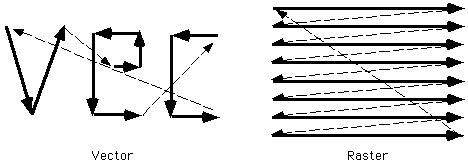
\includegraphics[width=0.8\linewidth]{images/scan.gif}
\caption{Scan comparison between vector graphics (left) and raster graphics (right). Source: \cite{vecvsras}}
\label{fig:vectorscan}
\end{figure}

Refresh rate depends on which type of phosphor is used. Some phosphor types fade out very quickly and needs refreshing 30-40 times per second. Special types of phosphor can last for several minutes.

The basic vector display is monochromatic. However, certain displays with color support exist. By using a shadow mask, that is a dotted plate that acts as a filter, between the electron guns and the screen, and having one electron gun for red, green and blue, RGB colors can be displayed on the screen.

Notable advantages with vector displays are:
\begin{itemize}
\item Since they are able to draw directly from one point to another, they do not suffer from artifacts such as aliasing and pixelation.
\item The entire screen is not updated every time, only the areas that the electron beam visits.

There are, however, some major disadvantages:
\begin{itemize}
\item Graphic detail on vector displays are very limited compared to raster screens, because of crude line drawings and often limited color support.
\item The refresh rate is also limited. When a bigger area of the screen is drawn, the screen starts to flicker more and more.
\item Irregular electron beam motion is slower than raster screens' predictable scanning.
\end{itemize} 

Vector displays are pretty much obsolete today, because of raster screens' inexpensiveness and support for graphics with a higher level of detail. Algorithms for graphics generation on raster screens are also much simpler than corresponding algorithms for vector screens.

\subsubsection{Oscilloscope}
As vector monitors are not easily available today, the group needed to find an alternative method of displaying vector graphics, preferrably without rasterization involved.
It is possible to modify a CRT monitor, so that one can manually control the deflectors, but this is quite cumbersome.
The other method is using an oscilloscope, which gives an easy interface to these deflectors.
This section will explain how to use the oscilloscope as a vector monitor.

The electron beam is deflected horizontally and vertically using electrostatic deflection. \cite{vector-monitor}

To be able to draw to a oscilloscope, the oscilloscope must support at least two input channels, and the ability to draw in X-Y mode.
In X-Y mode, two of the input channels (usually Ch1 and Ch2) governs the electron ray deflectors.
If the channels are provided a constant voltage, a dot will be displayed on the screen, in contrast to normal mode, where  a line would be drawn.

The voltage on channel 1 will normally decide the beam's horizontal position, and channel two, its vertical position.
To draw a line on the oscilloscope, one would need to repeatedly change the voltage of one or both channels back and forth.
Changing the voltage on only one channel will produce a horizontal or vertical line.
